\documentclass[oneside, 12pt]{book} 
\usepackage{multirow}

\title{Semantic parsing for Vietnamese Question Answering System}
\author{Name: Vu Xuan Tung\\
Student ID: 1310007 \\
School of Information Science}

\date{30/1/2014}

\usepackage[numbers]{natbib}
\usepackage[T5,T1]{fontenc}
\usepackage{amsmath}
\usepackage{graphicx}

\usepackage{indentfirst}
\usepackage[top=2.5cm, bottom=3cm, left=3cm, right=2cm]{geometry}

\linespread{1.3}
\setlength{\parindent}{1cm}
\setlength{\parskip}{6pt}

%\linespread{0.96}

\begin{document}
\fontsize{13pt}{18pt}\selectfont
\maketitle
\frontmatter
\usepackage{array}

\chapter*{\centering ADVISOR'S APPROVAL}
\noindent ``I hereby approve that the report in its current form is ready as a requirement for the Minor Research at Japan Advanced Institute of Science and Technology.''\\\\\\\\
Signature:...............................................................

\chapter*{\centering Abstract}
We apply a learning mechanism in to semantic parsing for Vietnamese. This kind of learning reduces the burden of providing supervision. The training data does not need to be carefully annotated. We only need some kind of "Question - Answer" data to train our model. 

%tables of contents
\tableofcontents

%\addcontentsline{toc}{chapter}{List of Figures}
%\listoffigures
%
%\addcontentsline{toc}{chapter}{List of Tables}
%\listoftables

\mainmatter

%introduction
\chapter{ Introduction}
\label{sec:introduction}

Semantic parsing is a very important process in Natural Language Processing. It converts a natural language sentence into a special meaning representation so that computer programs can read and process it. An effective way to do this task is using machine learning to build a model of relationship between natural language structure and formal representation structure. Unfortunately, most of the current approaches require very large amount of fully annotated data in order to obtain a good model. Annotated data means that for each input sentence of natural language, the corresponding representation is also provided. State-of-the-art methodologies often use statistical analysis to build the model and thus generally ill-perform with unseen data. Therefore, in order to get good results, they need to collect a large amount of annotated corpus. The annotation, however, is almost prepared manually and thus is difficult and time consuming. \cite{Zelle:1996:LPD:1864519.1864543}, \cite{Tang:2001:UMC:645328.650015}, \cite{Zettlemoyer05learningto}, \cite{Ge:2005:SSP:1706543.1706546}, \cite{Zettlemoyer07onlinelearning} and \cite{Wong07learningsynchronous} are examples of works in this category.

Recently, \citeauthor{Clarke:2010:DSP:1870568.1870571} in \cite{Clarke:2010:DSP:1870568.1870571} implemented a new learning paradigm aimed at alleviating the supervision burden. The algorithm is able to predict complex structures which only rely on a binary feedback. Borrowing the idea from these authors, we developed a question answering system for Vietnamese with suitable feature computations.

\subsection*{Related Work}
There has been not many works in Vietnamese semantic parsing. \citeauthor{Nguyen:2009:VQA:1681518.1683170} developed a question answering system for Vietnamese. The system enable users to query an ontological knowledge base using pattern matching. Although this kind of semantic parsing is simple and their testing data is small, the experiment shows promising results. 

The rest of this paper is organized as follow. Section \ref{sec:c-u} describes how natural language sentences are represented formally in our semantic parser. Section \ref{sec:model} illustrates the way we maintain the parsing model. We present our experiment result and discuss it in Section \ref{sec:experiment}. Finally, conclusion and future works are drawn in Section \ref{sec:conclusion}.

%Computer-understandable language
\chapter{Computer-understandable language}
\section{Computer-understandable language}
\label{sec:c-u}

The representation of meaning (the result of semantic parsing) depends on each system and need to be unified. In our system, the format of "Computer-understandable language" is composition of pre-defined functions. Each function has only one argument. For example, $capital(stateid("alaska"))$ is a CUL sentence, being a result of semantic parsing for "Thủ phủ của alaska là gì?" ("What is the capital of alaska?"). 

%Overview of VGQAS
\chapter{VGQAS overview}
\section{VGQAS overview}
\label{sec:system-overview}
The goal of the system is to provide users a smart machine, which can understand their questions and answer them properly. The main part considered here is semantic parsing. 

%Semantic parsing model
\chapter{Semantic parsing model}
\label{sec:model}
As mentioned, each parser system has a model for translating a natural language sentence to CUL sentence. In VGQAS, model consists of two parts: Word-Function feature calculator and Function-Function feature calculator.

\section{Word-Function feature vector calculator}
\label{sec:model.word-function}
This component is in charge of computing feature vector given a token and a function. Each function is configured to have a set of surface forms, which are typically associated with the function. The feature vector is calculated by comparing the token with these surface forms. Thus, the larger the number of surface forms is, the more accurate the feature vector is. Similar to \cite{Clarke:2010:DSP:1870568.1870571}, we restrict the number of surface forms per function. In our current experiment, there is average 1.39 words per functions, in comparison with 1.42 of \cite{Clarke:2010:DSP:1870568.1870571}.

The feature vector is generated based on lexical matching between token and surface forms. Many cases in Vietnamese, two words with lexical similarity may have the same meaning. For example "{\fontencoding{T5}\selectfont Ti\h\ecircumflex u bang" and "bang" both have meaning as "state". Similary, we have "con s\ocircumflex ng" and "s\ocircumflex ng" (river), "ng\d{o}n n\'ui" and "n\'ui", etc.} 
\subsection{Function - Function feature vector calculator}
\label{sec:model.function-function}
Suppose we need to compute the feature vector of $f_1$ and $f_2$ when we want to form $f_1(f_2(arg))$. $arg$ here is the argument of $f2$. The most important note is that returned type of $f_2$ must agree with one of argument types of $f_1$. The second feature is the vector of distance between the tokens mapped to two functions in the sentence. If the distance is small, they will have more chances to be composed. This is due to the usual speaking style of Vietnamese. Let us consider the following example: \\
 "{\fontencoding{T5}\selectfont con s\ocircumflex ng n\`ao ch\h{a}y qua ti\h\ecircumflex u bang missisipi?" ("what river runs through state mississippi?")}. There are at least two candidates for the result of semantic parser. They are illustrated in figure \ref{f-f.eg1} and figure \ref{f-f.eg2}. Between these two cases, our system tend to put more scores (higher value of features) on the first case. The intuition here is that, for example, "{\fontencoding{T5}\selectfont con s\ocircumflex ng}" comes before "{\fontencoding{T5}\selectfont ti\h\ecircumflex u bang}", the function $river$ is preferred to combine with $state$ to form $river(state(arg))$.
\begin{figure}[h]
\centering
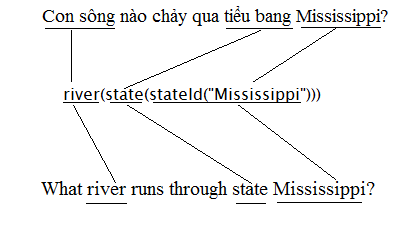
\includegraphics[scale=0.7]{eg-function-function-mapping1.png}
\caption{One result of parsing "{\fontencoding{T5}\selectfont con s\ocircumflex ng n\`ao ch\h{a}y qua ti\h\ecircumflex u bang missisipi?}"}
\label{f-f.eg1}
\end{figure}

\begin{figure}[ht!]
\centering
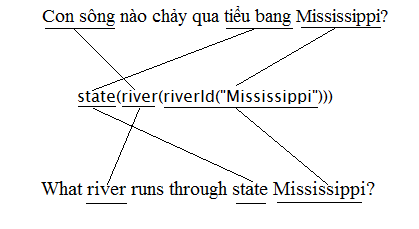
\includegraphics[scale=0.7]{eg-function-function-mapping2.png}
\caption{Another result of parsing "{\fontencoding{T5}\selectfont con s\ocircumflex ng n\`ao ch\h{a}y qua ti\h\ecircumflex u bang missisipi?}"}
\label{f-f.eg2}
\end{figure}

\subsubsection{A method of dynamic learning preference of functions compositions}
Until now, we have only one feature for describe the composition capacity of two functions. Another one is the feature which describe the compositional preferences of functions. A function is often composed with only a set some other functions. For example, $state$ function tends to receive $stateId$ function as its argument. In our approach, this feature is learned automatically through the running time of the system. 

Suppose $f1$ as a variable $p$ denoting how likely it will be composed with $f2$ to form $f1(f2(arg))$, and this composition appears in a result of semantic parser. By receiving the feedback from the outside world, we may have the answer that the result is correct or not.
\subsubsection*{If the result is correct}
In this case, we will increase the value of $p$ by formula \ref{increase-frequency}. It is clear that $p$ will be increased but it is always smaller than $M$, the maximum value of a feature.
\begin{equation}
\label{increase-frequency}
p = \frac{(p + 1)M}{M+1}
\end{equation}

\subsubsection*{If the result is wrong}
If the user says that he does not expect this answer, p needs to be decreased. Formula \ref{decrease-frequency} make the value of $p$ smaller. $p$ is also supposed to be greater or equal than $0$. 
\begin{equation}
\label{decrease-frequency}
p = \frac{p M}{M+1}
\end{equation}
\citeauthor{Clarke:2010:DSP:1870568.1870571} in \cite{Clarke:2010:DSP:1870568.1870571} also considered a feature indicating which logical symbols are usually composed together. Unfortunately, they did not clearly state the way of computing this kind of feature. If this task is done by manually configuring such feature when we define function, the result would be quite good. But that idea is not really positive with respective to scalability. Large number of functions will overwhelm annotators. 

\label{sec:experiment}
We use the Geoquery domain for evaluating our system. It consists of a database and Prolog query language for U.S. geographical facts. The corpus has 880 English tokenized queries; each query is paired with a Prolog query. We use Google Translate API to translate the English queries into Vietnamese ones. The translation contains many errors as the result of some word-to-word translations. We then manually correct each query to produce meaningful Vietnamese queries. 

Following the experiment in \cite{Clarke:2010:DSP:1870568.1870571}, we randomly select 250 queries for training, 250 other queries for testing from the above 880 queries. Our experiment is used to answer the following doubt:

\begin{enumerate}
  \item What are the effects of dynamic compositional preferences learning?
  \item How do two learning approaches of \cite{Clarke:2010:DSP:1870568.1870571} perform in our system?
\end{enumerate}

\subsection{What are the effects of dynamic compositional preferences learning?}
In this experiment, we use "Aggressive arrpoach" of machine learning in \cite{Clarke:2010:DSP:1870568.1870571}. The experiment result is described in table \ref{d-c-p-eff}. 

"No dynamic learning" row means that we do not use dynamic compositional preferences learning. When calculating the features for functions compositions, the second feature is the same as the first one. That means they are both computed based on the distance of two tokens.

It is clear from the table that the strategy of dynamic preferences computation improves the accuracy of the system by $4.4\%$ and $3.2\%$ for training data and testing data respectively. We also may wonder that if some set of questions is asked many times by users, how does this strategy perform? The last column of table \ref{d-c-p-eff} shows that if we repeatedly run the training data 10 times, then the final result on the training data is surprisingly $62\%$. In addition, if we run on testing data after running 10 times on training data, the accuracy for testing data is not significantly affected. It decreases by 1.6\%. 
\begin{table}[h] 
	\begin{center}
	    \begin{tabular}{| p{5cm} | c | c |}
	    \hline
	    Algorithm & Training set & Testing set \\ \hline
		No dynamic learning & 53.6\% & 51.6\%  \\ \hline
	    Dynamic learning & 58\% & 54.8\%  \\ \hline
	    Dynamic learning with repetition on training data & 62\% & 53.2\%  \\
	    \hline
	    \end{tabular}        
	\end{center}
	\scriptsize
	\caption{Accuracy of model on traing data and testing data. "No dynamic learning" means that we do not learn compositional preferences during running time of system. "Dynamic learning" means that we apply this kind of learning. in "Dynamic learning with repetition on training data", we run the system 10 times on training data; then testing data is also experimented}
    \label{d-c-p-eff}
\end{table}

\subsection{How do two learning approaches of \cite{Clarke:2010:DSP:1870568.1870571} perform in our system?}
We also implemented two learning mechanisms mentioned in \cite{Clarke:2010:DSP:1870568.1870571}. However, the "Direct Approach" or Binary classification did not successfully learn the weight vector. The learned vector contains negative coefficients. This is because the way we choose the feature of "Word-Function mapping" is simple, just being word matching. We need some semantics features which measure the semantic similarity between words. \citeauthor{Clarke:2010:DSP:1870568.1870571} in \cite{Clarke:2010:DSP:1870568.1870571} use Wordnet for this purpose. Unfortunately, we do not have Wordnet for Vietnamese. But we had some ideas for this problem. For instance, we can use word2vec, a tool of Google. This is left for our future works.

On the other hand, "Aggressive approach" performs quite well as illustrated in table \ref{d-c-p-eff}. Without machine learning, the result of both training data and testing data is around $20\%$.

\addcontentsline{toc}{chapter}{References}
\bibliographystyle{plainnat}
\bibliography{thesis}

\end{document}

